% This file was created by matlab2tikz.
%
%The latest updates can be retrieved from
%  http://www.mathworks.com/matlabcentral/fileexchange/22022-matlab2tikz-matlab2tikz
%where you can also make suggestions and rate matlab2tikz.
%

\documentclass[]{standalone}
\usepackage{amsmath}
\usepackage{graphicx}
\usepackage[pdf]{pstricks}
\usepackage{pgfplots}
\pgfplotsset{compat=newest}
\usepgfplotslibrary{fillbetween}
%% the following commands are needed for some matlab2tikz features
\usetikzlibrary{plotmarks}
\usetikzlibrary{arrows.meta}
\usepgfplotslibrary{patchplots}
\usetikzlibrary{decorations.text}
\usetikzlibrary{shapes.multipart}
\usetikzlibrary{external}
\tikzexternalize % activate!

\begin{document}
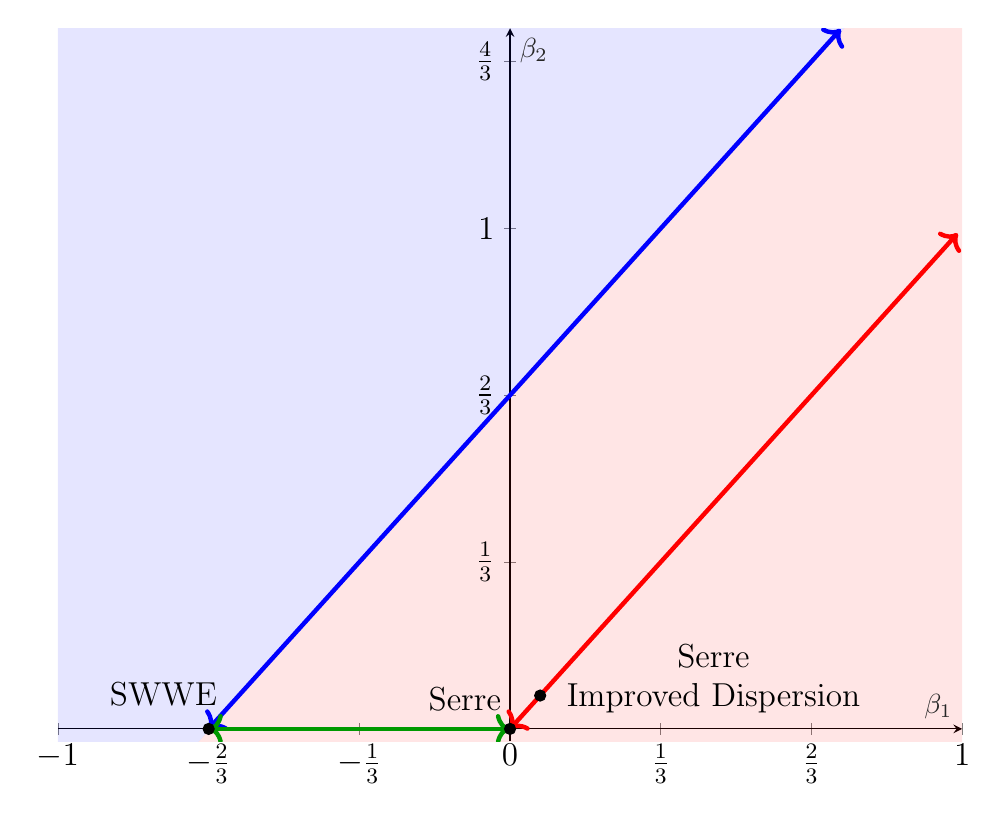
\begin{tikzpicture}[every text node part/.style={align=center}]
\tikzstyle{every node}=[font=\large]
\begin{axis}[%
width=4.521in,
height=3.566in,
at={(0.758in,0.481in)},
scale only axis,
axis lines=center,
xmin=-1,
xmax=1,
xtick={-1,-0.66666,-0.33333,0.33333,0.66666,1},
xticklabels = {$-1$,$-\frac23$,$-\frac13$,$\frac13$,$\frac23$,$1$},
extra x ticks=0,
xlabel style={font=\color{white!15!black}},
xlabel={$\beta_1$},
ymin=-0.025,
ymax=1.4,
ytick={0.33333,0.66666,1,1.33333},
yticklabels = {$\frac13$,$\frac23$,$1$,$\frac43$},
ylabel style={font=\color{white!15!black}},
ylabel={$\beta_2$},
axis background/.style={fill=white},
];
\addplot[only marks] coordinates {(0,0) (-0.6666,0) (0.06666,0.06666)};

\addplot[name path=Above,mark=none, white] coordinates {(-2,3) (2,3)};


\draw[<->,blue,ultra thick] (0.73133,1.398) --   (-0.66666,0) ;


\path[name path=Critical,thick] (1,1.66) --   (-2.66666,-2) ;

\addplot[name path=Below,mark=none, white] coordinates {(-2,-2) (2,-2)};
\addplot[blue,opacity=0.1] fill between[of=Above and Critical];
\addplot[red,opacity=0.1] fill between[of=Critical and Below];


\draw[<->,red,ultra thick] (0,0) --   (0.99,0.99) ;
\draw[<->,green!60!black,ultra thick] (-0.6666,0) --   (0,0) ;

\node[] at (axis cs: -0.1,0.06) {Serre};
\node[] at (axis cs: 0.45,0.1) {Serre \\Improved Dispersion};

\node[] at (axis cs: -0.7666,0.07) {SWWE};




\end{axis}

\end{tikzpicture}%

\end{document}